\documentclass[11pt,UTF8]{article}
\usepackage[no-math,cm-default]{fontspec}
\usepackage{amsmath}
\usepackage{amsthm}
\usepackage{amssymb}
\usepackage{xeCJK}
\usepackage{verbatim}
\usepackage{indentfirst}
\usepackage{syntonly}
\usepackage{fancyhdr}
\usepackage[unicode=true, colorlinks, linkcolor=black, anchorcolor=black, citecolor=black, urlcolor=black]{hyperref}
\usepackage{graphicx}
\usepackage[top = 1.2in, bottom = 1.2in, left = 1.3in, right = 1.3in]{geometry}
\usepackage{xcolor}
\usepackage{paralist}
\usepackage{ulem}
\usepackage{titlesec}
\usepackage{zhspacing}
\usepackage{booktabs}
\usepackage{multirow}
\usepackage{supertabular}
\usepackage{float}
\usepackage{soul}
\usepackage{longtable}
\usepackage{listings}
\usepackage{xcolor}
\usepackage{multicol}
\lstset{
    numbers=left, 
    numberstyle= \tiny, 
    keywordstyle= \color{ blue!70},
    commentstyle= \color{red!50!green!50!blue!50}, 
    frame=shadowbox, % 阴影效果
    rulesepcolor= \color{ red!20!green!20!blue!20} ,
    escapeinside=``, % 英文分号中可写入中文
    xleftmargin=2em,xrightmargin=2em, aboveskip=1em,
    framexleftmargin=2em
} 

\defaultfontfeatures{Mapping=tex-text}
%\setromanfont{Times New Roman}
%\newfontfamily\zhfont[BoldFont=Adobe Heiti Std]{Adobe Song Std}
\setmonofont[Scale=1]{Courier New}
\XeTeXlinebreaklocale "zh"
\XeTeXlinebreakskip = 0pt plus 1pt

\definecolor{hlcolor}{rgb}{0.9, 0.9, 0.9}
\sethlcolor{hlcolor}
\newcommand{\code}[1]{\texttt{\hl{#1}}}

\newcommand{\hlink}[1]{
	\footnote{\href{#1}{\textsl{\underline{#1}}}}
}
\renewenvironment{proof}{\noindent{\textbf{证明:}}}{\hfill $\square$ \vskip 4mm}
\newtheorem{conclusion*}{结论}
\newcommand{\conclusion}[1]{
	\begin{conclusion*}\textup{#1}\end{conclusion*}
}
\let\enumerate\compactenum
\let\endenumerate\endcompactenum
\let\itemize\compactitem
\let\enditemize\endcompactitem
\setlength{\pltopsep}{5pt}
\setlength{\parindent}{2em}
\setlength{\footskip}{30pt}
\setlength{\baselineskip}{1.3\baselineskip}
\renewcommand\arraystretch{1.2}

\lstset{language=C++,
	backgroundcolor=\color{hlcolor},
	extendedchars=false,
	basicstyle=\ttfamily,
	keywordstyle=\bfseries,
	commentstyle=\itshape\color{gray},
	escapeinside=`'}

\title{\fontsize{25pt}{\baselineskip}\textbf{图形学第一次作业\\[2ex]实验报告}}
\author{1600012938~周尚彦}
%\date{}

\pagestyle{fancy}
\renewcommand{\sectionmark}[1]{\markright{\thesection.\ #1}}
\renewcommand{\subsectionmark}[1]{}
%\fancyhead[C]{\small 湖南师大附中}
\fancyhead[L]{\small\slshape 图形学第一次作业}
\fancyhead[R]{\small\slshape\nouppercase{\rightmark}}
\fancypagestyle{plain}{\fancyhead{}\fancyfoot{}\renewcommand{\headrulewidth}{0pt}}

%\titleformat*{\section}{\fontsize{16pt}{\baselineskip}\bfseries}




\newcommand{\graph}[2]
{
\begin{figure}[H]
	\centering
	\includegraphics[width=\textwidth]{#1}
	\caption{#2}
\end{figure}
}

\begin{document}

\thispagestyle{plain}

\maketitle

%\setcounter{tocdepth}{1}
%\renewcommand{\contentsname}{\LARGE 目录}
\tableofcontents

\pagenumbering{arabic}
\setcounter{section}{0}

\section{代码与运行环境}
	\begin{itemize}
		\item 代码均在windows10 64位系统环境下使用python3.5.3编译运行。
		\item 调用第三方包Pillow中的Image读写图片,ImageDraw对图片进行绘制。
		\item 第五章作业使用了Pillow包内置的画线算法
	\end{itemize}
\newpage

\section{扫描线填充算法}
\subsection{算法流程}
	\begin{enumerate}
		\item 读入填充区域的顶点
		\item 使用Bresenham算法将各个顶点依次连接起来作为边界
		\item 枚举每个像素,若当前像素在区域内部且未被涂色则将其设定为为种子(使用累计角度法判断一个点是否在区域内部)
		\item 使用扫描线算法填充区域
	\end{enumerate}

\subsection{反走样}
	将每个边界附近的像素点均分成9个小像素点,判断每个点是否在多边形内部,之后加权求和算出像素点应有的灰度值。

\subsection{实验结果}
	\begin{figure}[H]
		\centering
		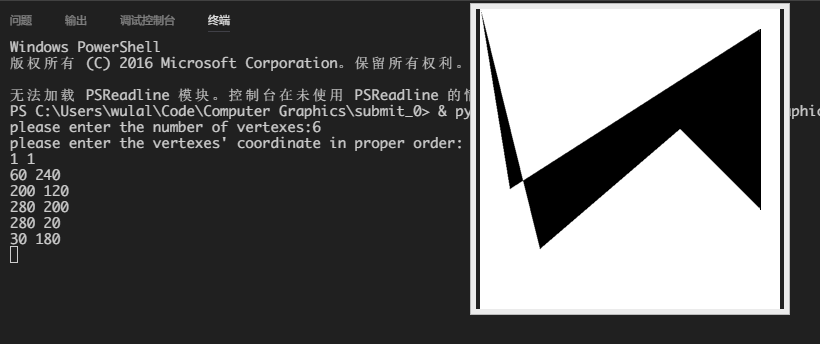
\includegraphics[width=\textwidth]{demo0.png}
		\caption{缩略图效果}\label{results}
	\end{figure}
	\begin{figure}[H]
		\centering
		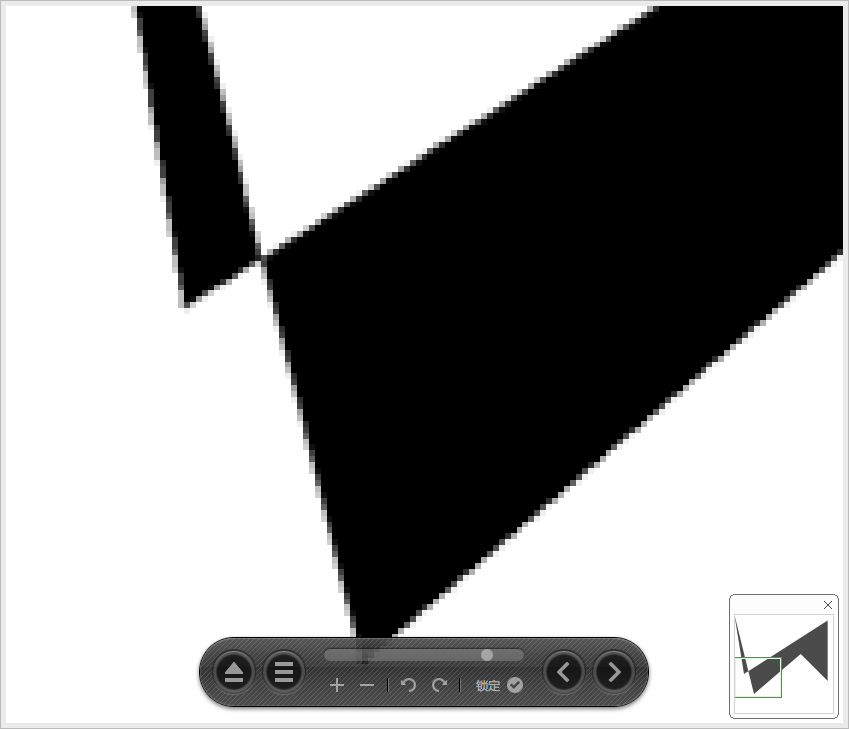
\includegraphics[width=\textwidth]{demo1.png}
		\caption{放大细节}\label{results}
	\end{figure}

\subsection{未解决问题}
	反走样时间花销很大,是否存在更好的方法?

	老师课件中给的例子(字母P)这样空心区域的边界如何表示?
\newpage
		

\section{直线反走样算法}
\subsection{算法流程}
	\begin{enumerate}
		\item 读入线段的端点
		\item 使用Bresenham算法画线,对直线附近的像素点使用加权区域采样的方法求出其灰度值
		\item 将每个像素点分为9个小像素点并分配以不同的权值,求出每个小像素点到直线的距离,若距离小于0.5则认为其在直线内部,加权求和最后得到该像素点的灰度值
	\end{enumerate}

\subsection{实验结果}
	\begin{figure}[H]
		\centering
		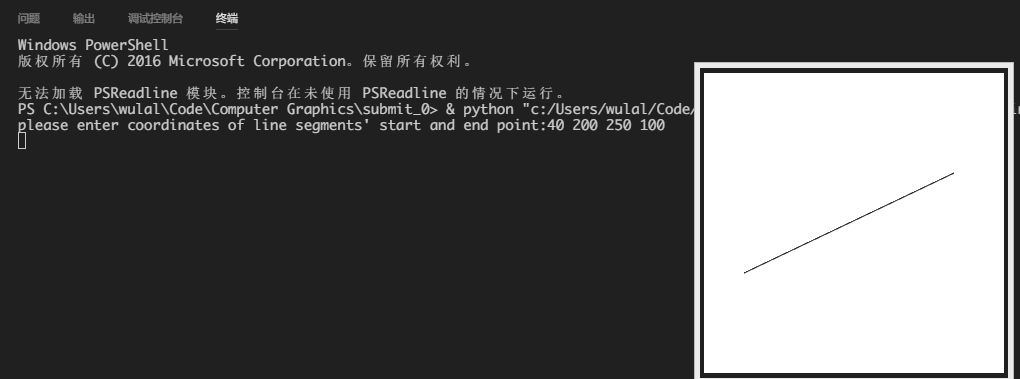
\includegraphics[width=\textwidth]{demo2.png}
		\caption{缩略图效果}\label{results}
	\end{figure}
	\begin{figure}[H]
		\centering
		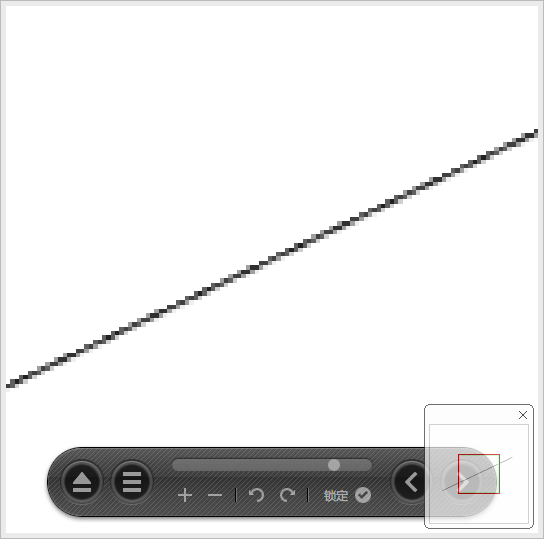
\includegraphics[width=\textwidth]{demo3.png}
		\caption{放大细节}\label{results}
	\end{figure}
\newpage

\section{Cohen-SutherLand算法}
\subsection{算法流程}
	\begin{enumerate}
		\item 读入矩形窗口的边界和线段的端点
		\item 对线段的端点进行编码,利用编码判断线段的可见性
		\item 利用编码求出第一个端点与边界所在直线的交点
		\item 修改第一个端点为此交点并重新编码,再次利用编码判断线段的可见性
		\item 利用编码求出第二个端点与边界所在直线的交点
		\item 使用红色线段标示不可见区域,绿色线段标识可见区域
	\end{enumerate}

\subsection{实验结果}
	\begin{figure}[H]
		\centering
		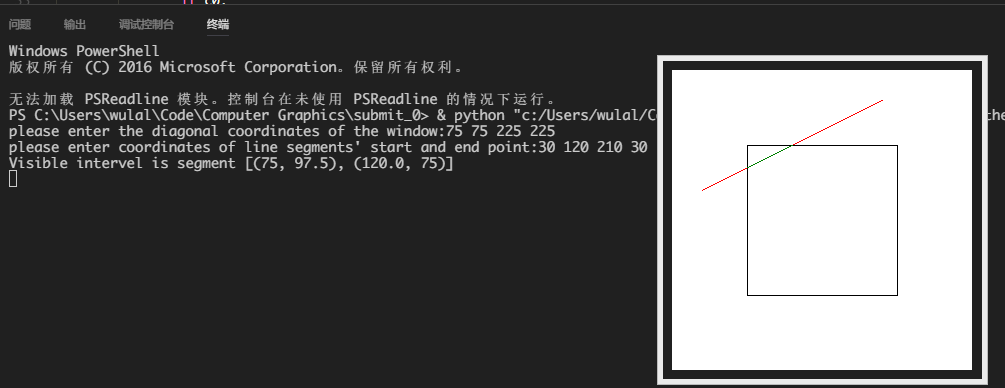
\includegraphics[width=\textwidth]{demo4.png}
		\caption{Demo0}\label{results}
	\end{figure}
	\begin{figure}[H]
		\centering
		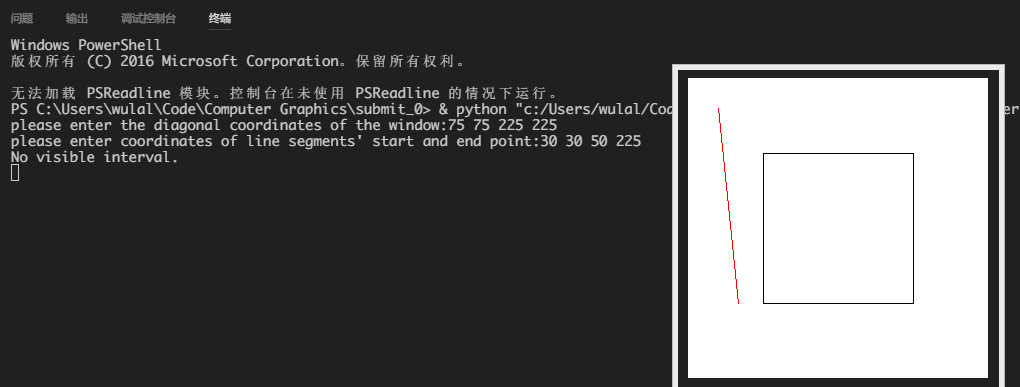
\includegraphics[width=\textwidth]{demo5.png}
		\caption{Demo1}\label{results}
	\end{figure}
\newpage

\section{Cyrus-Beck算法}
\subsection{算法流程}
	\begin{enumerate}
		\item 读入多边形窗口的顶点和线段的端点
		\item 求出每条边的法向量和中点
		\item 利用$n_i \bullet (p(t) - a_i)$列出不等式组并求解出$t$的最小最大值$l,r$
		\item 若$r \le l$则线段不可见,否则可见区域的交点为$p(l), p(r)$
		\item 使用红色线段标示不可见区域,绿色线段标识可见区域
	\end{enumerate}
\subsection{实验结果}
	\begin{figure}[H]
		\centering
		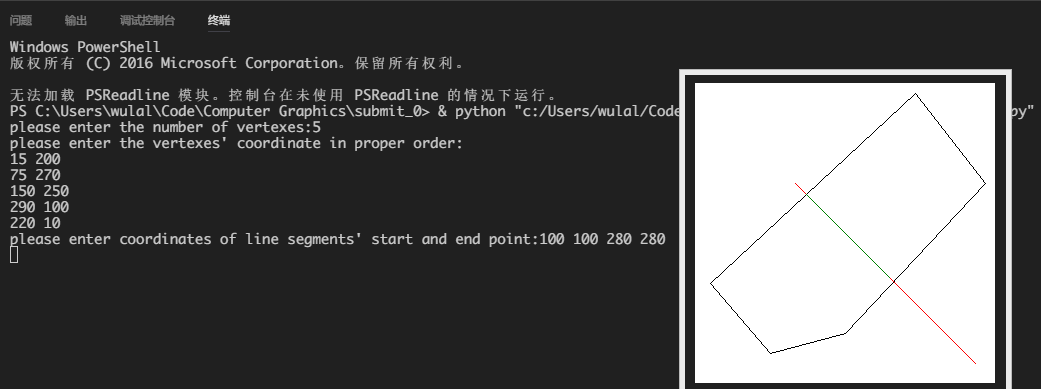
\includegraphics[width=\textwidth]{demo6.png}
		\caption{Demo}\label{results}
	\end{figure}
\end{document}
\newpage